\section{Optimization}
In this section, we'll talk more about optimization. 

\begin{definition}{Optimization}{}
    An \textbf{optimization} (for a compiler) is a version that produces programs that evaluate the same answer as the prior version, but are ``better'' on some cost metric.
\end{definition}

\subsection{Examples of Cost Metrics}
Some examples of cost metrics that we might want to improve on include 
\begin{itemize}
    \item \textbf{Time:} How long does it take for the program to run? 
    \item \textbf{Space:} How much process memory does the program use? 
    \item \textbf{Binary Size:} The size of the compiled binary, and the number of instructions.
    \item \textbf{Executed Instructions:} The overall number of instructions executed (compared to the total number of instructions). This is also similar to the number of jumps in the resulting assembly.  
\end{itemize}
\textbf{Remarks:}
\begin{itemize}
    \item The first two metrics -- time and space -- are generally the most important ones. 
    \item We might also care about properties like compile time, extensibility, debuggability, and platform independence, although these are harder to measure.
\end{itemize}

\subsection{High-Level Optimization Suggestions}
Some suggestions for optimizations include 
\begin{itemize}
    \item \textbf{Register Allocation:} Storing values in registers rather than in memory, since access to registers are generally faster than access to memory. 
    \item \textbf{Dead Code Elimination:} Remove code that the compiler can prove will never run.
    \begin{mdframed}
        (Example.) Consider the following code: 
        \begin{verbatim}
            if false 3 4 \end{verbatim}
        Here, we know for sure the \code{3} will never execute.
    \end{mdframed}
    This also includes things like removing unused variables from compilation. 

    \item \textbf{Constant Folding:} Evaluate ``what you can solve'' in the compiler. 
    \begin{mdframed}
        (Example.) Consider the following code:
        \begin{verbatim}
            (+ (* 2 3) input)\end{verbatim}
        Here, we know that \code{(* 2 3)} should be \code{6}, so this is basically equivalent to 
        \begin{verbatim}
            (+ 6 input)\end{verbatim}
    \end{mdframed}

    \item \textbf{Common Subexpression Elimination:} Eliminate repeated code in favor of a single instance of it. 
    \item \textbf{Memory Packing:} Eliminate unused memory due to alignment (e.g., struct alignment).
    \item \textbf{Loop Unrolling:} We can unroll a loop if we know that it has a constant bound. In other words, essentially hardcode all iterations.
    \begin{mdframed}
        (Example.) Consider the following code: 
        \begin{verbatim}
            (let (x 0) (loop (if (< x 3) (set! x (add1 x)) (break x))))\end{verbatim}
        This is equivalent to  
        \begin{verbatim}
            (let (x 0) (block 
                (set! x (add1 x))
                (set! x (add1 x))
                (set! x (add1 x))
            ))\end{verbatim}
    \end{mdframed}

    \item \textbf{Type-Directed Compilation:} We can remove some code that involves type checking if we know for sure that we're working with the correct types. 
    \begin{mdframed}
        (Example.) Consider the code 
        \begin{verbatim}
            (+ 1 (* input 2))\end{verbatim}
        While type checking is necessary for \code{(* input 2)}, it's probably not necessary for the plus expression since we can assume that both sides are numbers.
    \end{mdframed}

    \item \textbf{Peephole Optimization:} We can remove redundant move operations in the resulting assembly. 
    
    \item \textbf{Inlining Functions:} We can inline function calls, especially if we have a small one. 
    \begin{mdframed}
        (Example.) Consider the following function and resulting code: 
        \begin{verbatim}
            (fun (f x)
                <body>)
            (f 10)\end{verbatim}
        This could be functionally equivalent to  
        \begin{verbatim}
            (let (x 10) <body>)\end{verbatim}
    \end{mdframed}
    Note that we might need to consider things like recursion or other function calls in the function body, since that might prevent us for optimizing. 

    \item \textbf{Instruction Selection:} We can also possibly exploit the structure of our code. 
    \begin{mdframed}
        (Example.) Consider the following code: 
        \begin{verbatim}
            (if (< x 10) ... ...)\end{verbatim}
        Generally, our compiler would put either \code{true} or \code{false} into \code{rax}, and then evaluate \code{rax} when deciding where to jump. However, in this particular code, we can probably just conditionally jump on the spot.  
    \end{mdframed}
\end{itemize}

\subsection{Optimization: Register Allocation}
Let's consider the following code: 
\begin{verbatim}
    (let (n (+ 5 9))
        (let (m (+ 2 3))
            (let (x (+ n 1))
                (let (y (+ m 2))
                    (+ x y)))))\end{verbatim}

The corresponding assembly\footnote{With tag checks removed to make the assembly more concise.}, along with the corresponding code from the above, is shown below.
\begin{verbatim}
    sub rsp, 40
      mov rax, 10
      mov [rsp + 0], rax    ; LHS of (+ 5 9)
      mov rax, 18
      add rax, [rsp + 0]

      mov [rsp + 0], rax    ; Variable n in (let (n ...))

      mov rax, 4
      mov [rsp + 8], rax    ; LHS of (+ 2 3)
      mov rax, 6
      add rax, [rsp + 8]

      mov [rsp + 8], rax    ; Variable m

      mov rax, [rsp + 0]    ; Variable n lookup 
      mov [rsp + 16], rax   ; LHS of (+ n 1)
      mov rax, 2
      add rax, [rsp + 16]

      mov [rsp + 16], rax   ; Variable x

      mov rax, [rsp + 8]    ; Variable m lookup 
      mov [rsp + 24], rax   ; LHS of (+ m 2)
      mov rax, 4
      add rax, [rsp + 24]

      mov [rsp + 24], rax   ; Variable y 

      mov rax, [rsp + 16]   ; Variable x lookup 
      mov [rsp + 32], rax
      mov rax, [rsp + 24]   ; Variable y lookup 
      add rax, [rsp + 32]
    add rsp, 40\end{verbatim}
One thing to notice immediately is that we reused some memory locations. One example is \code{[rsp + 8]}, which is where we stored both a temporary for addition and a value associated with a variable. We can generalize how many memory locations we ultimately \emph{will} use by using the \code{depth} function. In particular, if $\code{depth(expr)} \leq \text{Available Registers}$, then we can avoid memory entirely.

\bigskip 

There are two questions we should now consider.
\begin{enumerate}
    \item (\code{x86\_64}.) What registers should we use?
    \begin{mdframed}
        We can use the registers \code{rbx}, \code{r12}, \code{r13}, \code{r14}, which are callee-saved registers. Note that we aren't using \code{r15} because this register is specifically the heap pointer.
    \end{mdframed}
    \item (Design.) How should we implement this?
    \begin{mdframed}
        We can create a \code{Loc} \emph{enum} that holds either a register or a stack location (offset). Then, our environment can be represented by \code{HashMap<String, Loc>}.

        \bigskip 

        Suppose we have a list of registers that we can use. We can create a \code{get\_loc} function which takes a stack index and returns the new location to be used; this might look something like 
        \begin{verbatim}
    let regs = [...];
    get_loc(si):
        if si < regs.size():
            return regs[si];
        else:
            return Stack(si - regs.len());\end{verbatim}
        Then, we can use this location to update the environment, like 
        \begin{verbatim}
    ... 
    | ELet(x, val, body) => {
        env.update(x, get_loc(si));
    }\end{verbatim}
        Note that, while this is an \emph{improvement} to how our program is compiled, this can still be made a \emph{lot better}. Some other implementation notes to consider include: 
        \begin{itemize}
            \item We need to add code to save and restore registers in function definitions.
            \item We need to compute stack size based on \code{depth - available registers}.
        \end{itemize}
        Some improvements we could make to what we have so far include 
        \begin{itemize}
            \item Registers for outer bindings and stack for inner bindings. 
            \item Frequency matters. 
            \item Precompute registers and locations for all variables and temporaries across functions. 
            \item Are we using the minimal number of locations? (e.g., is the depth minimal?)
        \end{itemize}
    \end{mdframed} 
\end{enumerate}
\textbf{Remark:} The register allocation algorithm we're talking about, which uses an idea similar to \code{depth}, is similar to the \emph{Sethi-Ullman algorithm}.

\subsubsection{High Level Steps}
At a high level, we aim to answer the following questions:
\begin{itemize}
    \item The first step is to find the minimal number of locations needed to store all the working variables in an expression.
    \item What pairs of variables must be stored (or must be ``live'') at the same time? 
\end{itemize}

\subsubsection{The Minimal Number of Locations}
Consider the following program: 
\begin{verbatim}
    (let (b 4)
        (let (x 10)
            (let (i (if input 
                        (let (z 11) (+ z b))
                        (let (y 9) (+ y 1))))
                (let (a (+ i 5))
                    (+ a x)))))\end{verbatim}
To answer the second question, note that 
\begin{itemize}
    \item \code{i} and \code{x} need storage at the same time.
    \item \code{a} and \code{b} do not need storage at the same time\footnote{Notice how we only use \code{b} once: in the \code{if}-expression. After that, we don't use \code{b} again.}. 
\end{itemize}
How many memory locations are needed? We'll look at the program from the \emph{end} to the beginning.
\begin{itemize}
    \item We first begin by looking at what variables are in use at the end. In this case, \code{a} and \code{x} are in use. The set of all variables in use is \[\{a, x\}.\]
    \item We're going to go back ``up'' the program. When we get to a \code{let}-bindings, we're going to remove it from the set of variables that are in use right now. In the next level, we're \emph{using} \code{i} and \code{x}, but we aren't using \code{a} here since \code{a} is being created. The set of all variables in use is \[\{i, x\}.\]
    \item The \code{if}-expression is more interesting. We need to consider both branches of the \code{if}-expression. Note that, in this step, \code{i} is being created, so we don't have access to \code{i} yet.
    \begin{itemize}
        \item Looking at the end of the ``else'' branch, at the body of the \code{let} binding, notice how \code{y} is being used. \code{x} is still around. The set of all variables in use is \[\{y, x\}.\]
        \item Looking at the end of the ``then'' branch, at the body of the \code{let} binding, notice how \code{z} and \code{b}\footnote{Even though \code{b} is defined at the top, this is the first time we're seeing \code{b} in use.} are in use. As usual, \code{x} is still around. The set of all variables in use is \[\{z, b, x\}.\]

    \end{itemize}
    \item At the \code{let}-binding for \code{i} (\emph{not} in the body), we no longer have \code{z} or \code{y}, and \code{i} is being initialized here (so we aren't using \code{i} here). Thus, this gives us the variables in use \[\{x, b\}.\] 
    \item Moving ``up'' the program to the \code{let}-binding for \code{x}, we now only have the variables in use $\{x\}$. 
    \item Finally, moving ``up'' the program to the \code{let}-binding for \code{b}, we have the variables in use $\emptyset$. 
\end{itemize}
This information is telling us what variables need to be stored at the same time. Something we can do with this information is turn this into a \textbf{graph} where there's an edge between two variables \emph{if} they're in use at the same time. 
\begin{center}
    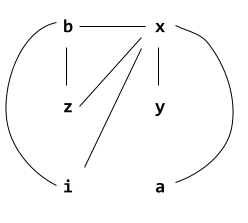
\includegraphics[scale=0.6]{assets/loc_use1.png}
\end{center}
This is a graph where if there are two variables that had to be live at the same time, then there is an edge. How do we make it so we can have a set of locations where each variable can be assigned to a register that's different from all the things it conflicts with? This problem is known as \textbf{graph coloring}. The idea is that we want to find $k$ colors assigning $1 \hdots k$ to each node such that $k$ is minimal and no edge has the same index for both nodes. A coloring for this graph is 
\begin{center}
    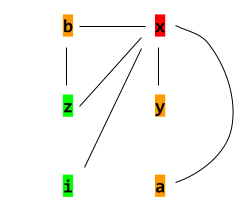
\includegraphics[scale=0.6]{assets/loc_use2.png}
\end{center}
We only need 3 colors! In terms of what our compiler would output, we would end up with the environment 
\begin{verbatim}
    {x: 1, b: 2, y: 2, a: 2, z: 3, i: 3}\end{verbatim}
In other words, \code{x} gets abstract location 1, \code{b} gets abstract location 2, and so on. Note that this makes a few assumptions: 
\begin{itemize}
    \item All intermediates are carefully named and used (no useless temporaries).
    \item Assuming all temporaries are explicit, this could replace \code{depth(e)}. Note that this means \emph{simple constants!}
    \item All variables are distinctly named (although we can rename all non-distinct names if needed).
\end{itemize}

\subsubsection{Algorithm}
The algorithm for this process is as follows: 
\begin{itemize}
    \item Visit last, or innermost, expression first. THis means recurse, then working with result. 
    \item Track set of variables we have seen used, then remove from set at the let-bindings.
\end{itemize}
So, going back to the example code, we have the following set of active variables.
\begin{verbatim}
    (let (b 4)                                  ; {}
        (let (x 10)                             ; {b}
            (let (i (if input                   ; {b, x}
                        (let (z 11) (+ z b))    ; {z, b, x}
                        (let (y 9) (+ y 1))))   ; {y, x}
                (let (a (+ i 5))                ; {i, x}
                    (+ a x)))))                 ; {a, x}\end{verbatim}
For each pair of active variables that appear at the same time, we draw an edge between them in the graph.

\subsubsection{Restrictions}
One of the main restrictions of the algorithm for register allocation is simply temporary values: what do we do with register allocation for temporary values that don't have any names?

\subsection{Intermediate Representation}
Let's consider the following program:
\begin{verbatim}
    (+ (- 5 input) (* input (if (> 0 input) 1 -1)))\end{verbatim}
Below is a transformed version of the program where every nested expression that would have introduced a temporary is now a \code{let}-bound variable. 
\begin{verbatim}
    (let (tmp 1 (- t input))
        (let (tmp 2 (> 0 input))
            (let (tmp3 (if tmp2 1 -1))
                (let (tmp4 (* input tmp3))
                    (+ tmp1 tmp4)
                )
            )
        )
    )\end{verbatim}
This makes the order of operations very explicit. Notice that it's very clear that we're doing left-to-right operation. This process also makes code generation for operations a lot easier, since everything is already stored on the stack or in a register. 

\begin{mdframed}
    (Example.) Perform the transformation on the function 
    \begin{verbatim}
    (fun (sumsquares x y)
        (+ (* x x) (* y y)))\end{verbatim}

    \begin{mdframed}
        As mentioned, we want to break our complex expression into much simpler types. We can accomplish this by defining any computations into \code{let}-bindings. This gives us 
        \begin{verbatim}
    (fun (sumsquares x y)
        (let (val (* x x))
            (let (val2 (* y y))
                (+ val val2)
            )
        )
    )\end{verbatim}
    \end{mdframed}
\end{mdframed}
This transformation is fairly common, and there is a fairly standard algorithm for this transformation that takes every non-trivial or non-atomic (basically, everything that's not a literal value) and puts them in a \code{let}-binding. 

\subsubsection{Different Grammar Forms}
There are two types of grammars we want to consider. 
\begin{itemize}
    \item \textbf{A-Normal Form:} This is essentially our grammar as is. This cares about scope, binding, order or evaluations, and so on. 
    
    \begin{verbatim}
        <expr> := <number> | <id> | true | false | nil 
            | (+ <expr> <expr>)
            | (- <expr> <expr>)
            | (if <expr> <expr> <expr>)
            | (break <expr>)
            | ... 
            | (let (<id> <expr>) <expr>)
            | ... \end{verbatim}
    \item \textbf{ANF-Restricted Grammar:} This grammar is effectively the transformed grammar; that is, given our A-Normal Form, we can transform it into a more restricted version. We'll denote this as \code{AExpr}.
    \begin{verbatim}
        <val> := <number> | <id> | true | false | nil 
        <expr> := (+ <val> <val>) 
            | (pair <val> <val>) 
            | (if <val> <block> <block>)
            | (break <val>)
        <block> := (let (<id> <expr>) <block>)
            | (loop <block>)
            | (break <block>+)
            | ... 
            | <expr>
            | <val>\end{verbatim}
        This is restricted in the sense that the grammar is broken up into three different groups (productions). You have expressions (\code{<expr>}) that form blocks (\code{<block>}). Blocks have expressions in them that can perform calculations; so, we can think of \code{<expr>} as something that performs a calculation of some type (e.g., binary operations, creating a new pair, and so on). All the arguments to these expressions that do calculations must be primitive values or identifiers.  
\end{itemize}
\textbf{Remark:} Loops are an interesting case to think about here. 

\subsubsection{Going from Normal to Restricted}
How do we create an algorithm that transforms code written under one grammar to code written in the restricted grammar? Note that this is a very standard algorithm, so we'll mainly gain some intuition. One choice to make is whether we want to introduce a new \code{enum} for ANF expressions. For example, is it worth it to introduce a bunch of new \code{enum}s like shown below?
\begin{verbatim}
    enum Val {
        VNum,
        VId(String),
        ...
    }

    enum AExpr {
        APlus(...),
        APair(...),
        ... 
    }

    enum Block {
        BLet(...),
        ...
    }\end{verbatim}

In any case, we can write a few functions to facilitate the conversion process.
\begin{itemize}
    \item \verb|anf_to_val(e: &Expr) -> Val|: Converts an A-Normal Expression Form to a literal value under the ANF-Restricted Expression Form.
    \item \verb|anf_to_expr(e: &Expr) -> AExpr|: Converts an A-Normal Expression Form to a computation expression under the ANF-Restricted Expression Form.
    \item \verb|anf_to_block(e: &Expr) -> Block|: Converts an A-Normal Expression Form to a block expression under the ANF-Restricted Expression Form. 
\end{itemize}

\subsubsection{ANF to Value}
Let's suppose we want to implement 
\begin{verbatim}
    fn anf_to_val(e: &Expr) -> Val {
        match e {
            ...
        }
    }\end{verbatim}

\begin{itemize}
    \item For an expression \code{e} like \code{Number(n)}, we can trivially return \code{VNum(n)}.
    \item For an expression \code{e} like \code{Plus(e1, e2)}, this becomes more complicated. This will involve a nested plus expression, and we should return an identifier that we can use later. Note that \code{e1} and \code{e2} may be complicated expressions, but we want them to be \code{Val}s as well. So, we'll probably need to do some recursive calls to ideally break \code{e1} and \code{e2} down into \code{let}-bindings. 
    \begin{verbatim}
        Plus(e1, e2) => {
            let (v1, b1) = anf_to_val(e1);
            let (v2, b2) = anf_to_val(e2);
            // Assume new_label() is a function that returns a new identifier.
            let new_name = new_label(); 
            // This isn't Rust syntax, but basically we want all the bindings from 
            // b1, all the bindings from b2, and our new binding in this vector.
            (VId(new_name), vec![...b1, ...b2, (new_name, APlus(v1, v2))])
        }\end{verbatim}
    Notice how we're returning a tuple. The first element is the identifier that will store the result of the evaluation of this expression. However, we also need to return list of \code{let}-bindings we need to eventually stick in front of \emph{this} identifier in order for it to work (otherwise, the identifier won't be bound). So, we should modify the function return type: 
    \begin{verbatim}
    fn anf_to_val(e: &Expr) -> (Val, Vec<(String, AExpr)>) { ... }\end{verbatim}
\end{itemize}

\subsection{Intermediate Representation}
\subsubsection{Rust AST}
Given what we've just discussed, the Rust representation of A-Normal Form and ANF-Restricted Form might look something like 
\begin{verbatim}
    pub enum AVal {
        Num(i32),
        True,
        False,
        Id(String),
    }

    pub enum AExpr {
        Plus(Box<AVal>, Box<AVal>),
        Eq(Box<AVal>, Box<AVal>),
        Lt(Box<AVal>, Box<AVal>),
        Print(Box<AVal>),
        Set(String, Box<AVal>),
        Call1(String, Box<AVal>),
        Call2(String, Box<AVal>, Box<AVal>),
        Pair(Box<AVal>, Box<AVal>),
        Fst(Box<AVal>),
        Snd(Box<AVal>),
        Break(Box<AVal>),
        Loop(Box<ABlock>),
        If(Box<AVal>, Box<ABlock>, Box<ABlock>),
        Val(Box<AVal>),
    }

    pub enum ABlock {
        Let(String, Box<AExpr>, Box<ABlock>),
        Block(Vec<ABlock>),
        Op(Box<AExpr>),
    }\end{verbatim}

\subsubsection{A Problem With Loops}
Consider the following function:
\begin{verbatim}
    (fun (range low high)
        (let (n high)
            (let (lst nil)
                (loop
                    (if (= n low) (break lst)
                        (block
                            (set! n (+ n -1))
                            (set! lst (pair n lst)))
                    )
                )
            )
        )
    )
\end{verbatim}
Converting the above function, which is written in A-Normal Form, to ANF-Restricted Form, yields:
\begin{verbatim}
    (fun (range low high)
        (let (n high)
            (let (lst nil)
                (loop
                    (let (%t_0 (= n low))
                        (if %t_0 (break lst)
                            (block
                                (let (%t_1 (+ n -1)) (set! n %t_1))
                                (let (%t_2 (pair n lst)) (set! lst %t_2)))
                        )
                    )
                )
            )
        )
    )\end{verbatim}
Note that the \verb|%| identifiers are just the convention we're using for temporaries. Let's now consider all interfering variables, which we can do by considering all variables inside-out. 
\begin{verbatim}
    (fun (range low high)
        (let (n high)           ; low, high
            (let (lst nil)                  ; n, low
                (loop
                    (let (%t_0 (= n low))           ; lst, n, low, t_0
                        (if %t_0 (break lst)        ; n, lst, t_0
                            (block
                                (let (%t_1 (+ n -1)) (set! n %t_1))         ; t_1, n, lst
                                (let (%t_2 (pair n lst)) (set! lst %t_2)))  ; t_2, lst, n
                        )
                    )
                )
            )
        )
    )\end{verbatim}
Notice that we end up with the set of variables $\{\code{n}, \code{low}, \code{lst}, \verb|t_0|, \verb|t_1|, \verb|t_2|, \code{high}\}$. A graph representing this would look like 
\begin{center}
    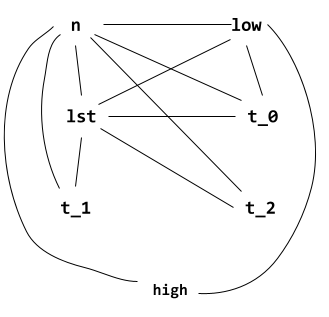
\includegraphics[scale=0.6]{assets/loc_pt2.png}
\end{center}

\begin{mdframed}
    (Exercise.) How would the graph change if we swapped the order of the \code{set!} lines?

    \begin{mdframed}
        \underline{Suggestion:} Because the last use of \code{lst} would be in the first \code{set!} instead of the last line, there wouldn't be an edge between \code{lst} and \code{t\_1}. 

        \bigskip 

        But, one thing to keep in mind is that the \code{set!} is in a loop. So, \code{lst} needs to be in scope for the remainder of the block statement. Otherwise, a temporary could be assigned to the same register that was being used for \code{lst}. 
    \end{mdframed}
\end{mdframed}
\textbf{Remarks:}
\begin{itemize}
    \item Remember that our algorithm just went from the end to beginning, but now we need to consider what identifiers have been defined outside of the loop. 

    \item The issue with loops is that you have implicit backedges from the last expression in the loop to the beginning of the loop. We don't have names associated with these loops, which makes things difficult since we have names in the first place so we know where everything is. 
\end{itemize}

\subsubsection{A Rewrite of the Grammar}
How do we rewrite our grammar to account for loops? 
\begin{verbatim}
    pub enum Val {
        Num(i32),
        True,
        False,
        Id(String),
    }


    pub enum Expr {
        Plus(Box<Val>, Box<Val>),
        Eq(Box<Val>, Box<Val>),
        Lt(Box<Val>, Box<Val>),
        Print(Box<Val>),
        Call1(String, Box<Val>),
        Call2(String, Box<Val>, Box<Val>),
        Pair(Box<Val>, Box<Val>),
        Fst(Box<Val>),
        Snd(Box<Val>),
        Val(Box<Val>),
    }


    pub enum Step {
        Label(String),
        If(Box<Val>, String, String)
        Goto(String),
        Do(Expr),
        Set(String, Expr)
    }


    pub struct Block {
        pub steps: Vec<Step>,
    }\end{verbatim}
Some things to notice here: 
\begin{itemize}
    \item Rather than expressing our program as loops with breaks, we'll express them as labels and gotos. 
    \item In the \code{if}-condition, the first \code{String} is the label to jump to if the condition is true; the last \code{String} is the label to jump to if the condition is false. 
    \item So, whereas ANF is about scope and temporary variables, this is about control flow. Essentially, we're iteratively getting closer to assembly.
\end{itemize}
Here, we introduce the concept of \textbf{intermediate representation}. With the above new representation, we have the following intermediate representation:
\begin{verbatim}
    range(low,high) {
        n <- high
        lst <- nil
       loop_0:
        %t_0 <- n == low
        if %t_0 thn_3 els_4
       thn_3:
        rax <- lst
        goto end_1
        goto ifend_2
       els_4:
        %t_1 <- pair(n, lst)
        lst <- %t_1
        %t_2 <- n + -1
        n <- %t_2
        rax <- n
        goto ifend_2
       ifend_2:
        goto loop_0
       end_1:
        return rax
    }\end{verbatim}
Note that this is the compiled output of the \code{range} function, not in x86\_64. Some things to note: 
\begin{itemize}
    \item There's no nesting of expressions anymore. There's no notion of labels being inside other labels. 
    \item Lots of IRs have support for functions (including things like function scope, blocks within functions, etc.), but leave the actual calling convention to the language. 
    \item The pipeline we would have is that surface syntax turns into ANF, and then ANF turns into IR. It's possible to do everything in one pass, but it's easier to do it in two passes.
    \item In this example of \code{range}, \code{rax} is now our designated answer variable, and we expect all lines before the \code{return rax} line to store the answer into \code{rax} (similar to what our compiler does right now).
\end{itemize}
With that said, running through the IR representation from last to start, the variables in use are: 
\begin{verbatim}
    range(low,high) {           ; {}
        n <- high               ; n
        lst <- nil              ; n, lst 
       loop_0:                  ; n, lst
        %t_0 <- n == low        ; t_0, n, lst 
        if %t_0 thn_3 els_4     ; t_0, n, lst  
       thn_3:                   ; lst 
        rax <- lst              ; rax, lst 
        goto end_1              ; rax 
        goto ifend_2            ; <empty for now>
       els_4:                   ; n, lst, t_1
        %t_1 <- pair(n, lst)    ; n, lst, t_1
        lst <- %t_1             ; lst, n, t_1
        %t_2 <- n + -1          ; t_2, n 
        n <- %t_2               ; t_2, n 
        rax <- n                ; n, rax 
        goto ifend_2            ; <empty for now>
       ifend_2:                 ; <empty for now>
        goto loop_0             ; <empty for now>
       end_1:                   ; rax 
        return rax              ; rax
    }\end{verbatim}
Any time you reach a \code{goto}, any variables that are used at the jump target are copied over to the \code{goto}. In any case, we should not use this information to construct the graph needed to figure out how many registers we need to allocate. In particular, at these three instructions,
\begin{verbatim}
    %t_2 <- n + -1          ; t_2, n 
    n <- %t_2               ; t_2, n 
    rax <- n                ; n, rax \end{verbatim}
there's no edge between \code{lst} and \code{t\_2}. This means that we could potentially store \code{lst} and \code{t\_2} into the same register, losing a possible important value. So, we need to run this same algorithm over and over until none of the sets change (i.e., when saturation occurs). Running through the algorithm again gives us: 
\begin{verbatim}
    range(low,high) {           ; {}                ; 
        n <- high               ; n                 ; 
        lst <- nil              ; n, lst            ; 
       loop_0:                  ; n, lst            ; 
        %t_0 <- n == low        ; t_0, n, lst       ; 
        if %t_0 thn_3 els_4     ; t_0, n, lst       ; 
       thn_3:                   ; lst               ; 
        rax <- lst              ; rax, lst          ;
        goto end_1              ; rax               ; 
        goto ifend_2            ; <empty for now>   ; n, lst
       els_4:                   ; n, lst, t_1       ; 
        %t_1 <- pair(n, lst)    ; n, lst, t_1       ; 
        lst <- %t_1             ; lst, n, t_1       ; 
        %t_2 <- n + -1          ; t_2, n            ; lst 
        n <- %t_2               ; t_2, n            ; lst 
        rax <- n                ; n, rax            ; lst
        goto ifend_2            ; <empty for now>   ; n, lst
       ifend_2:                 ; <empty for now>   ; n, lst
        goto loop_0             ; <empty for now>   ; n, lst
       end_1:                   ; rax               ; 
        return rax              ; rax               ; 
    }\end{verbatim}
Note that the last column are the variables \emph{added} to the variables mentioned in the second columns. Anyways, after running this algorithm again, we reach saturation -- we don't find any additional variables that need to be added. This gives us a complete graph that we can use to determine what registers can be allocated.

\subsection{Flow Analysis}
Let's consider the following code, 
\begin{verbatim}
    (let (curr lst)
        (let (total 0)
            (loop
                (if (= lst nil) (break total)
                    (block
                    (set! total (+ total (fst lst)))
                    (set! lst (snd lst)))))))\end{verbatim}
How can we use flow analysis to reduce the amount of tag checking generated in the final assembly?

\subsubsection{The \code{check} Instruction}
An idea we want to do is to make tag checks explicit with \code{check} steps: which checks can we remove? One new step we can introduce in the intermediate representation is 
\begin{verbatim}
    check <some bool expr>\end{verbatim} 
The semantics are simple: if the check is true, then everything continues as normal. Otherwise, an error is thrown.
\begin{mdframed}
    (Example.) \code{check sametag(curr, nil)} checks to see if \code{curr} has the same tag as \code{nil}. Something we've incorporated into our compiler is the \code{isnum(x)} and \code{isbool(x)} checks, which checks to see if the expression $x$ is a number or boolean, respectively.
\end{mdframed}
With this said, the corresponding intermediate representation of the above code is 
\begin{verbatim}
sum(lst) {
    start0:     curr <- lst
    start1:     total <- 0
    loop_0:     check sametag(curr, nil)
    loop_1:     %t_0 <- curr == nil
    loop_2:     if %t_0 thn_0 els_0
    thn_0:      rax <- total
    thn_1:      goto end_0
    thn_2:      goto ifend_0
    els_0:      check isnonnilpair(curr)
    els_1:      %t_1 <- fst curr
    els_2:      check isnum(total)
    els_3:      check isnum(%t_1)
    els_4:      %t_2 <- total + %t_1
    els_5:      total <- %t_2
    els_6:      check isnonnilpair(curr)
    els_7:      %t_3 <- snd curr
    els_8:      curr <- %t_3
    els_9:      rax <- curr
    els_10:     goto ifend_0
    ifend_0:    goto loop_0
    end_0:      return rax
}\end{verbatim}
We can use flow analysis to analyze how data flows through a program. We can use this information to identify variables that hold values at different points in the program, and how these values change over time. For our purposes, we wish to use flow analysis to reduce the amount of unnecessary tag checking. Using the \code{check} instruction that was mentioned, we can do just this.

\newpage 
\thispagestyle{noheader}
\newgeometry{left=0.1in,right=0.1in,top=0.2in,bottom=0.5in}
\subsubsection{A Flow Analysis Walkthrough}
The flow analysis we'll do starts from the beginning and goes to the end (this is known as \emph{forward analysis}). The information we'll keep track of are the \emph{potential} tags. Let's analyze each line of the intermediate representation. For each line executed, we consider what possible tag value each variable can represent. The potential tags are \textbf{N}umbers, \textbf{B}ooleans, \textbf{Nil}, and \textbf{P}airs. At any point in the program, each variable can hold a set of these possible types. Let $A = \{N, B, \text{Nil}, P\}$ be the set of all types.

\begin{center}
    \begin{tabular}{p{2.5in}|p{0.48in}|p{0.82in}|p{0.48in}|p{0.48in}|p{0.48in}|p{0.48in}|p{0.48in}|p{0.48in}}
        IR & \code{lst} & \code{curr} & \code{total} & $t_0$ & $t_1$ & $t_2$ & $t_3$ & \code{rax} \\ 
        \hline  
        \hline 
        \verb|start0:  curr <- lst|                 & A & $\to A$  &   &   &   &   &   &   \\
        \hline
        \verb|start1:  total <- 0|                  & A & A  & $\to N$ &   &   &   &   &   \\
        \hline
        \verb|loop_0:  check sametag(curr, nil)|    & A  & $\to \{\text{Nil}, P\}$ & N &   &   &   &   &   \\
        \hline
        \verb|loop_1:  %t_0 <- curr == nil|         & A & $\{\text{Nil}, P\}$ & N & $\to B$ &   &   &   &   \\
        \hline
        \verb|loop_2:  if %t_0 thn_0 els_0|         & A & $\{\text{Nil}, P\}$  & N & B &   &   &   &   \\
        \hline
        \verb|thn_0:   rax <- total|                & A & \{\text{Nil}, P\} & N & B &   &   &   & N \\
        \hline
        \verb|thn_1:   goto end_0|                  & A & \{\text{Nil}, P\} & N & B &   &   &   & N \\
        \hline
        \verb|thn_2:   goto ifend_0|\footnote[100]{}     &    &   &   &   &   &   &   &   \\
        \hline
        \verb|els_0:   check isnonnilpair(curr)|\footnote[101]{}  & A & $\{\text{Nil}, P\} \to P$  & N & B &   &   &   &   \\
        \hline
        \verb|els_1:   %t_1 <- fst curr|            & A & P & N & B & $\to A$ &   &   &   \\
        \hline
        \verb|els_2:   check isnum(total)|          & A & P & $N \to N$ & B & $\to A$ &   &   &   \\
        \hline
        \verb|els_3:   check isnum(%t_1)|           & A & P & N & B & $A \to N$ &   &   &   \\
        \hline
        \verb|els_4:   %t_2 <- total + %t_1|        & A & P & N & B & N & $\to N$  &   &  \\
        \hline
        \verb|els_5:   total <- %t_2|               & A & P & $N \to N$ & B & N & N  &   &    \\
        \hline
        \verb|els_6:   check isnonnilpair(curr)|    & A & $P \to P$ & N & B & N & N  &   &    \\
        \hline
        \verb|els_7:   %t_3 <- snd curr|            & A & P & N & B & N & N  & $\to A$ &   \\
        \hline
        \verb|els_8:   curr <- %t_3|                & A & $P \to A$ & N & B & N & N  & A &   \\
        \hline
        \verb|els_9:   rax <- curr|                 & A & A & N & B & N & N & A & $\to A$ \\
        \hline
        \verb|els_10:  goto ifend_0|                & A & A & N & B & N & N & A & A \\
        \hline
        \verb|ifend_0: goto loop_0|                 & A & A & N & B & N & N & A & A \\
        \hline
        \verb|end_0:   return rax|                  &   &   &   &   &   &   &   &   \\
    \end{tabular}
\end{center}
\textbf{Remarks:}
\begin{itemize}
    \item At (100), we have dead code. So, nothing needs to be filled out.
    \item At (101), we can copy the tag information we have from the \code{goto} instruction which jumps to this line. In this case, we copied this information from the line \code{loop\_2}.
    \item In general, we can copy the information from the \code{goto} to the target label. This is especially important when we have a \code{goto} that goes to a label that's \emph{before} where the \code{goto} occurred.
\end{itemize}
At \code{goto loop\_0}, we now perform a backwards jump back to the label \code{loop\_0} and perform additional forward analysis with the information we found prior to the \code{goto}. These tags are denoted by red.
\begin{center}
    \begin{tabular}{p{2.5in}|p{0.48in}|p{0.82in}|p{0.48in}|p{0.48in}|p{0.48in}|p{0.48in}|p{0.48in}|p{0.48in}}
        IR & \code{lst} & \code{curr} & \code{total} & $t_0$ & $t_1$ & $t_2$ & $t_3$ & \code{rax} \\ 
        \hline  
        \hline 
        \verb|start0:  curr <- lst|                 & A & $\to A$  &   &   &   &   &   &   \\
        \hline
        \verb|start1:  total <- 0|                  & A & A  & $\to N$ &   &   &   &   &   \\
        \hline
        \verb|loop_0:  check sametag(curr, nil)|    & A  & $\textcolor{red}{A} \to \{\text{Nil}, P\}$ & N & \textcolor{red}{$\to B$} & \textcolor{red}{$\to N$}  & \textcolor{red}{$\to N$} & \textcolor{red}{$\to A$} & \textcolor{red}{$\to A$} \\
        \hline
        \verb|loop_1:  %t_0 <- curr == nil|         & A & $\{\text{Nil}, P\}$ & N & $\to B$ & \textcolor{red}{N}  & \textcolor{red}{N} & \textcolor{red}{A} & \textcolor{red}{A} \\
        \hline
        \verb|loop_2:  if %t_0 thn_0 els_0|         & A & $\{\text{Nil}, P\}$  & N & B & \textcolor{red}{N}  & \textcolor{red}{N} & \textcolor{red}{A} & \textcolor{red}{A} \\
        \hline
        \verb|thn_0:   rax <- total|                & A & \{\text{Nil}, P\} & N & B & \textcolor{red}{N}  & \textcolor{red}{N} & \textcolor{red}{A} & $\textcolor{red}{A} \to N$ \\
        \hline
        \verb|thn_1:   goto end_0|                  & A & \{\text{Nil}, P\} & N & B & \textcolor{red}{N}  & \textcolor{red}{N} & \textcolor{red}{A} & N \\
        \hline
        \verb|thn_2:   goto ifend_0|     &    &   &   &   &   &   &   &   \\
        \hline
        \verb|els_0:   check isnonnilpair(curr)|\footnote[102]{}  & A & $\{\text{Nil}, P\} \to P$  & N & B & \textcolor{red}{N}  & \textcolor{red}{N} & \textcolor{red}{A} & \textcolor{red}{A} \\
        \hline
        \verb|els_1:   %t_1 <- fst curr|            & A & P & N & B & $\to A$ &   &   &   \\
        \hline
        \verb|els_2:   check isnum(total)|          & A & P & $N \to N$ & B & $\to A$ &   &   &   \\
        \hline
        \verb|els_3:   check isnum(%t_1)|           & A & P & N & B & $A \to N$ &   &   &   \\
        \hline
        \verb|els_4:   %t_2 <- total + %t_1|        & A & P & N & B & N & $\to N$  &   &  \\
        \hline
        \verb|els_5:   total <- %t_2|               & A & P & $N \to N$ & B & N & N  &   &    \\
        \hline
        \verb|els_6:   check isnonnilpair(curr)|    & A & $P \to P$ & N & B & N & N  &   &    \\
        \hline
        \verb|els_7:   %t_3 <- snd curr|            & A & P & N & B & N & N  & $\to A$ &   \\
        \hline
        \verb|els_8:   curr <- %t_3|                & A & $P \to A$ & N & B & N & N  & A &   \\
        \hline
        \verb|els_9:   rax <- curr|                 & A & A & N & B & N & N & A & $\to A$ \\
        \hline
        \verb|els_10:  goto ifend_0|                & A & A & N & B & N & N & A & A \\
        \hline
        \verb|ifend_0: goto loop_0|                 & A & A & N & B & N & N & A & A \\
        \hline
        \verb|end_0:   return rax|                  &   &   &   &   &   &   &   &   \\
    \end{tabular}
\end{center}

\restoregeometry
\newpage 

\textbf{Remark:}
\begin{itemize}
    \item At (102), note that we're not directly copying $N$ from \code{thn\_1} to \code{els\_0}. Rather, we're copying the tag information from the \code{goto} instruction that jumps to this line. 
\end{itemize}
Let's consider the lines \verb|els_2: check isnum(total)| and \verb|els_6: check isnonnilpair(curr)|. Based on the forward analysis, these two lines of code are useless. Likewise, \verb|els_0: check isnonnilpair(curr)| could be \emph{optimized} (not removed) to check if \code{curr} is \code{nil}.

\subsubsection{In Summary}
In summary, the idea behind flow analysis is that there's really two steps: 
\begin{enumerate}
    \item Do the analysis and gather information 
    \item Rescan the program with that information and change the program to remove/optimize any code as needed. 
\end{enumerate}
The corresponding \textbf{control flow graph} looks like 
\begin{center}
    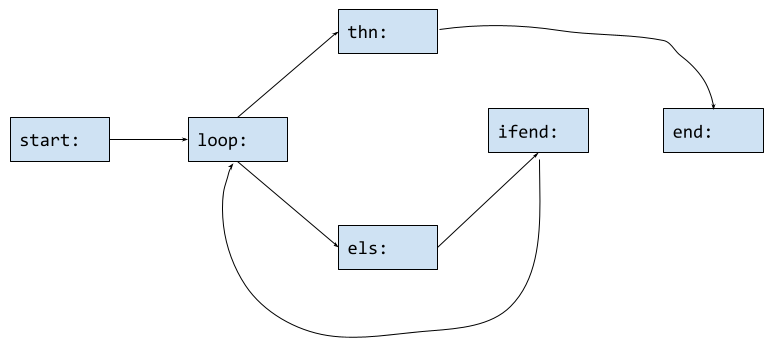
\includegraphics[scale=0.5]{assets/analysis_flow_graph.png}
\end{center}
At the start, we have a bunch of instructions. This eventually leads to a loop. In the \code{thn} branch, we go straight to the end since we have the dead code. In the \code{els} branch, we eventually get to the \code{ifend} statement where we end up going to the loop.

\thispagestyle{noheader}
\newgeometry{left=0.1in,right=0.1in,top=0.2in,bottom=0.5in}

\subsubsection{Another Flow Analysis Walkthrough}
Consider the following program: 
\begin{verbatim}
    (fun (same_at vec1 vec2 i)
        (= (index vec1 i) (index vec2 i)))\end{verbatim}
We'll perform another flow analysis\footnote{Note that this IR representation was generated by hand.}, again by starting from the beginning and going to the end. The information we'll keep track of are the \emph{potential} tags. Our tags are now slightly more refined; in particular, we now have the set of tags, 
\[\text{tag} := Z | \text{Pos} | \text{Neg} | B | V | \text{Nil}\]
Here, \code{Z} means the number zero, \code{Pos} means positive number, \code{Neg} means negative number. We also have \code{B} for boolean, \code{V} for vector, and \code{Nil} for nil. Once again, we let $A$ represent the set of all possible tags. We also introduce $N = \{Z, \text{Pos}, \text{Neg}\}$ for numbers\footnote{Note that there's no overlaps in this set; we either have negative numbers, positive numbers, and zero.}. 

\begin{center}
    \begin{tabular}{p{2.5in}|p{0.65in}|p{0.65in}|p{1.25in}|p{0.65in}|p{0.65in}|p{0.65in}}
        IR & \code{vec1} & \code{vec2} & \code{i} & $t_0$ & $t_1$ & \code{rax} \\ 
        \hline 
        \verb|start0: check isnonnilvec(vec1)|      & $\to V$ &   &   &   &   &   \\
        \verb|start1: check isnum(i)|               & V &   & $\to N$ &   &   &   \\
        \verb|start2: check i >= 0|                 & V &   & $N \to \{Z, \text{Pos}\}$ &   &   &   \\
        \verb|start3: check i < len(vec1)|          & V &   & $\{Z, \text{Pos}\} \to \{Z, \text{Pos}\}$ &   &   &   \\
        \verb|start4: %t_0 <- vec1[i]|              & V &   & $\{Z, \text{Pos}\}$ & $\to A$ &   &   \\
        \verb|start5: check isnonnilvec(vec2)|      & V & $\to V$ & $\{Z, \text{Pos}\}$ & A &   &   \\
        \verb|start6: check isnum(i)|               & V & V & $\{Z, \text{Pos}\}$ & A &   &   \\
        \verb|start7: check i >= 0|                 & . & . & . & . &   &   \\
        \verb|start8: check i < len(vec2)|          & . & . & . & . &   &   \\
        \verb|start9: %t_1 <- vec2[i]|              & . & . & . & . &   &   \\
        \verb|start10:check sametag(%t_0, %t_1)|    &   &   &   &   &   &   \\
        \verb|start10:rax <- %t_0 == %t_1|          &   &   &   &   &   &   \\
        \verb|return rax|                           &   &   &   &   &   &   \\
    \end{tabular}
\end{center}
Note that, at \code{start7}, at our second pass, we can either reduce this to just checking \code{true}, or just deleting the check altogether.

\subsubsection{Abstract Domains}
We're now incorporating forward analysis with some numeric range analysis. We can call these types of analysis abstract domains. We have seen three different abstract domains for analysis: 
\begin{itemize}
    \item \code{Set<String>} for liveliness analysis (for register allocation).
    \item \code{Dict<String, Set<Tag>>} for forward data analysis. 
\end{itemize}
There were two different types of tags: 
\begin{itemize}
    \item \code{Z | P | N}: information about numbers (positive, negative, etc.)
    \item \code{N | B | Nil | P}: other relevant tag information.
\end{itemize}
How do we unify these domains? We can consider ideas like: 
\begin{itemize}
    \item Frequency for variable use.
    \item Frequency of branches. 
    \item Ranges of numbers. 
    \item Booleans as true or false.
    \item Lengths of vectors (if we have constants, e.g., setting the tag to be the length of the vector).
\end{itemize}

\restoregeometry
\newpage 